\documentclass[12pt]{article}
\usepackage{fullpage}
\usepackage{multicol}
\usepackage{fontspec}
\usepackage{graphicx}
\usepackage{setspace}
\doublespacing
\setmainfont{OpenDyslexicAlta}
\title{Algebra Test 1 Review}
\newcommand{\blk}{\underline{\hspace{0.5in}}}
\begin{document}
%\maketitle
\center{\section*{Algebra Test 2}}
\center{\section*{Work in your NOTEBOOK, AND SHOW ALL WORK!}}
%\begin{multicols}{2}
\begin{enumerate}
	\item Solve for $x$: $2x=12$
	
	\item Solve for $x$: $4x=9$
	
	\item Solve for $x$: $x+6=14$
	
	\item Solve for $x$: $x+8=3$
	
	\item Solve for $x$: $2x+3=21$
	
	\item Solve for $x$: $3x-8 = 2x+5$
	
	\item Multiply out and simplify: $\displaystyle \frac{2}{3} \times \frac{7}{5}$
	
	\item Divide and simplify: $\displaystyle \frac{3}{5} \div \frac{7}{4}$
	
	
	\pagebreak
	\item In the right triangle below $a=3$ and $b=4$, solve for $c$:
	
	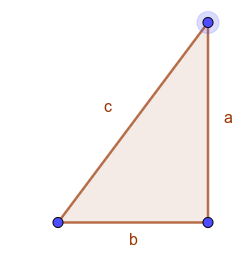
\includegraphics[width=2.5in]{345triangle.png}
	
	\item Calculate: $\displaystyle \sqrt{36}$
	
	\item Calculate: $\displaystyle \sqrt{3^2 + 4^2}$
	
	\item Calculate: $ \sqrt{0.25}$

	\item Is $x=10$ a solution of $2x+3=25$?
	
	\item Is $x=3$ a solution of $x^2-2x-3=0$?
		
	\item You buy a meal for yourself and 3 of your friends.  The meals all cost the same amount.  You pay with a \$20 bill and receive a \$5 bill for change.
	\begin{enumerate}
		\item 	Write an equation for this situation (using materials or not)
		\item Solve the equation
		\item How much did each meal cost?
	\end{enumerate}

	\item Write out a statement of the Pythagorean Theorem.
	
	\pagebreak
	
	\item (Extra Credit): Multiply and simplify: $\displaystyle \frac{12}{20}$

	\item (Extra Credit): Solve: $\displaystyle \frac{2}{3} x + 1 = 9$
	
	\item (Extra Credit): Write a paragraph about your biography mathematician.  Include at least 3 sentences.
\end{enumerate}
%\end{multicols}
\end{document}